\chapter{Analiza poprawności wersji kwantowej}
\label{chap:quantum_probability_results}

W niniejszym rozdziale przeprowadzono analizę poprawności kwantowej wersji algorytmu Dijkstry wykorzystującej algorytm wyszukiwania minimum Dürra-Høyera. Analizie poddano cztery rodzaje grafów: graf rzadki, graf o średniej gęstości, graf gęsty oraz przypadek szczególny. W pierwszej kolejności przeanalizowano skuteczność samego algorytmu wyszukiwania minimum, a następnie skuteczność całego algorytmu Dijkstry. Wyniki przedstawiono osobno dla wersji z limitem liczby operacji oraz bez limitu. W dalszej części rozdziału przeanalizowano zależność pomiędzy błędnym znalezieniem minimum a poprawnością końcowego wyniku algorytmu Dijkstry.

\section{Skuteczność wyszukiwania minimum z limitem}

\begin{figure}[H]
    \centering
    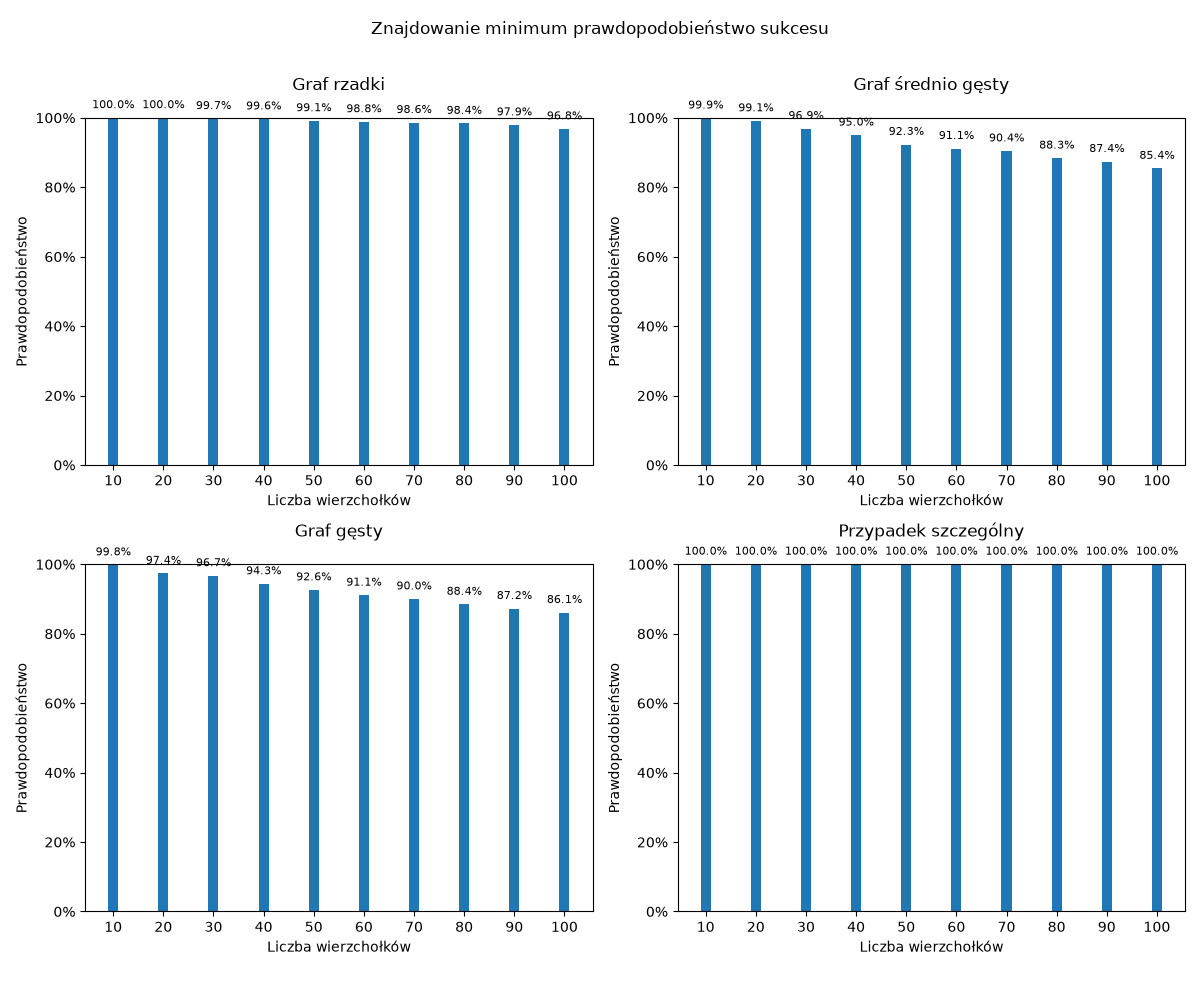
\includegraphics[width=0.95\columnwidth]{images/documentation/quantum_prob/quantum_prob_min_time_limit.png}
    \caption{Prawdopodobieństwo poprawnego znalezienia minimum przez algorytm Dürra-Høyera z limitem liczby operacji.}
    \label{fig:quantum_prob_min_time_limit}
\end{figure}

Na rys.~\ref{fig:quantum_prob_min_time_limit} przedstawiono prawdopodobieństwo poprawnego znalezienia minimum przy zastosowaniu limitu liczby operacji.

Najbardziej widoczny jest spadek prawdopodobieństwa poprawnego wyszukania minimum wraz ze wzrostem liczby wierzchołków. Zjawisko to występuje przede wszystkim dla grafów o średniej gęstości oraz grafów gęstych. Dla grafów o małej liczbie wierzchołków skuteczność pozostaje bliska $100\%$, a dla większych grafów stopniowo maleje. W przypadku grafu rzadkiego spadek prawdopodobieństwa poprawnego wyniku jest znacznie mniejszy. Skuteczność pozostaje bardzo wysoka nawet dla największych grafów. Natomiast przypadek szczególny zachowuje się inaczej od pozostałych typów grafów. Dla wszystkich analizowanych rozmiarów algorytm odnajduje poprawne minimum. 

Uzyskane wyniki pokazują, że wpływ limitu nie zależy wyłącznie od liczby wierzchołków. Znaczenie ma też struktura grafu i odległości między wierzchołkami, które stanowią dane wejściowe dla algorytmu wyszukiwania minimum.

\begin{figure}[H]
    \centering
    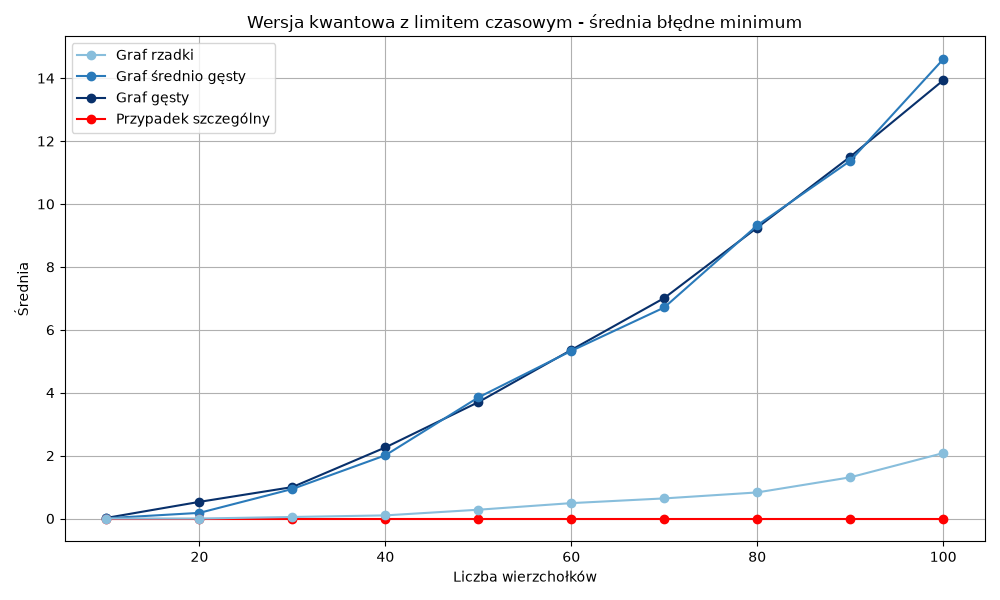
\includegraphics[width=0.95\columnwidth]{images/documentation/quantum_prob/quantum_min_time_limit.png}
    \caption{Średnia liczba błędnych wyszukiwań minimum w zależności od liczby wierzchołków dla konfiguracji z limitem.}
    \label{fig:quantum_min_time_limit}
\end{figure}

Na rys.~\ref{fig:quantum_min_time_limit} przedstawiono średnią liczbę błędnych wyszukiwań minimum w zależności od liczby wierzchołków. Wraz ze wzrostem rozmiaru grafu liczba błędów zauważalnie rośnie przede wszystkim dla grafów o średniej gęstości oraz grafów gęstych. Dla grafu rzadkiego wartości pozostają niewielkie, natomiast w przypadku szczególnym błędne wyszukiwania minimum nie występują. 

\section{Skuteczność algorytmu Dijkstry z limitem}

\begin{figure}[H]
    \centering
    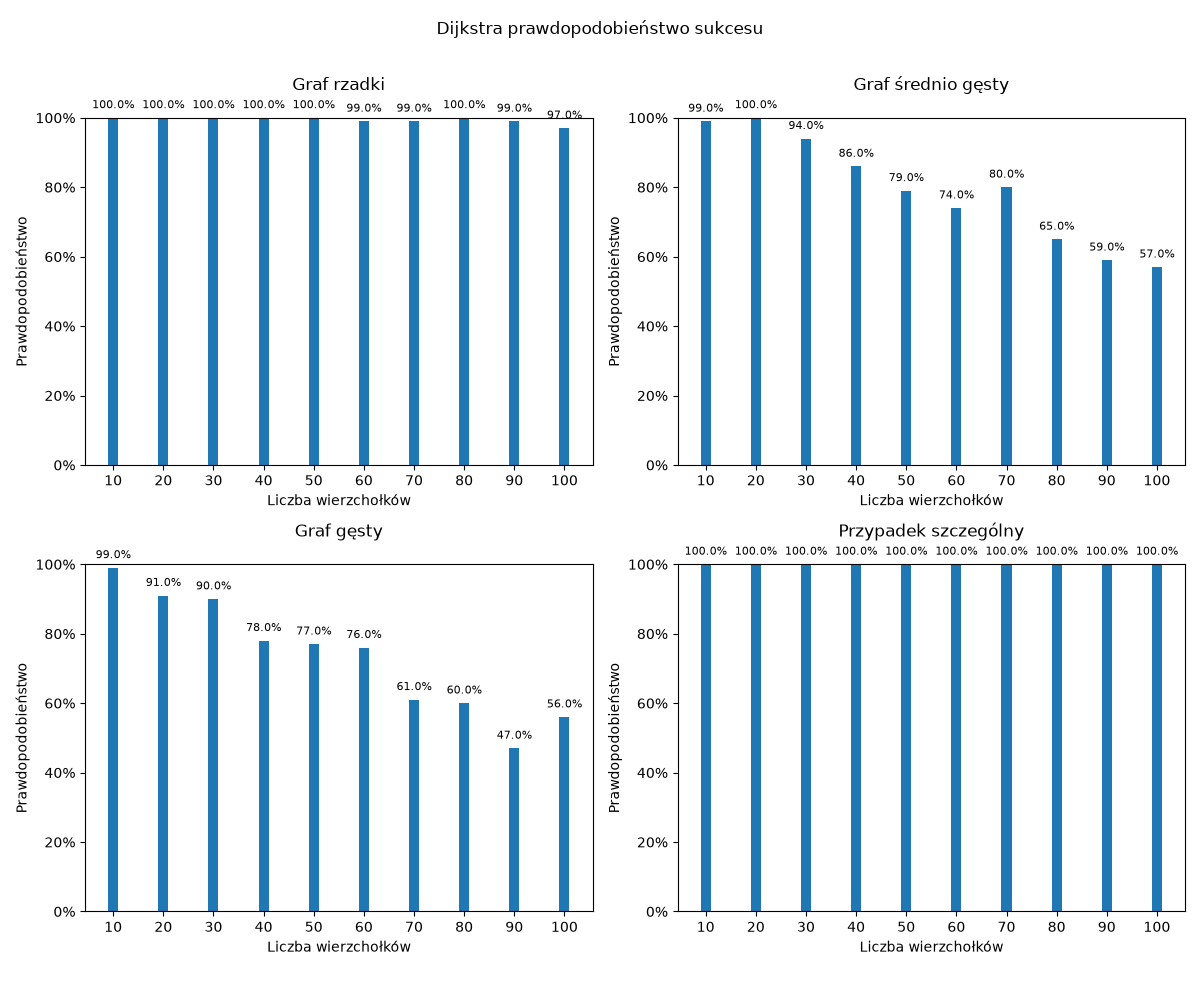
\includegraphics[width=0.95\columnwidth]{images/documentation/quantum_prob/quantum_prob_dijkstra_time_limit.png}
    \caption{Prawdopodobieństwo otrzymania poprawnego wyniku kwantowej wersji algorytmu Dijkstry z limitem liczby operacji.}
    \label{fig:quantum_prob_dijkstra_time_limit}
\end{figure}

Na rys.~\ref{fig:quantum_prob_dijkstra_time_limit} przedstawiono skuteczność całego algorytmu Dijkstry w wersji z limitem liczby operacji.

Widoczna jest podobna zależność jak w przypadku samego wyszukiwania minimum, ale spadek prawdopodobieństwa sukcesu jest znacznie większy. Dla grafu rzadkiego algorytm zachowuje wysoką poprawność ale dla grafów średnio gęstych oraz gęstych skuteczność maleje znacznie szybciej wraz ze wzrostem liczby wierzchołków.

Różnica ta wynika z wielokrotnego wykonywania wyszukiwania minimum podczas jednego uruchomienia algorytmu Dijkstry. Nawet jeżeli pojedyncze wyszukiwanie minimum ma wysokie prawdopodobieństwo sukcesu, każde kolejne wywołanie stanowi dodatkową możliwość wystąpienia błędu. Dlatego wraz ze wzrostem rozmiaru grafu coraz bardziej widoczna staje się różnica pomiędzy skutecznością pojedynczej operacji wyszukiwania minimum a skutecznością całego algorytmu Dijkstry. 


\section{Skuteczność wyszukiwania minimum bez limitu}

\begin{figure}[H]
    \centering
    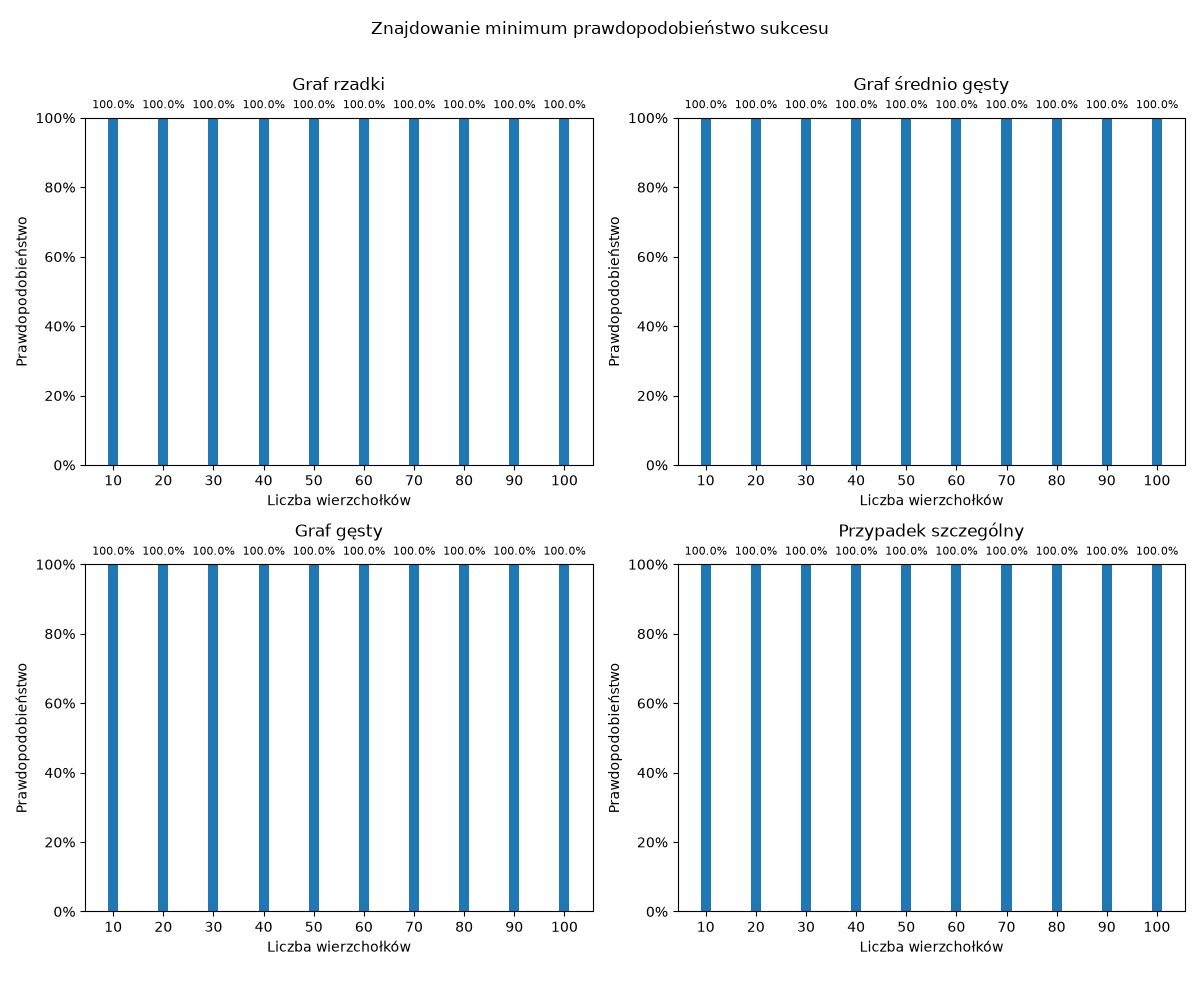
\includegraphics[width=0.95\columnwidth]{images/documentation/quantum_prob/quantum_prob_min_no_time_limit.png}
    \caption{Prawdopodobieństwo poprawnego znalezienia minimum przez algorytm Dürra-Høyera bez limitu liczby operacji.}
    \label{fig:quantum_prob_min_no_time_limit}
\end{figure}

Na rys.~\ref{fig:quantum_prob_min_no_time_limit} przedstawiono skuteczność wyszukiwania minimum bez ograniczenia liczby operacji.

W tej wersji dla wszystkich typów grafów oraz wszystkich badanych rozmiarów otrzymano pełną skuteczność. W porównaniu do wersji z limitem widać, że ograniczenie liczby wykonywanych operacji odpowiada za obserwowane wcześniej błędy. Gdy algorytm wyszukiwania minimum może wykonać nieograniczoną ilość prób, zwiększanie liczby wierzchołków nie prowadzi do pogorszenia poprawności wyszukiwania minimum.

\section{Skuteczność algorytmu Dijkstry bez limitu}

\begin{figure}[H]
    \centering
    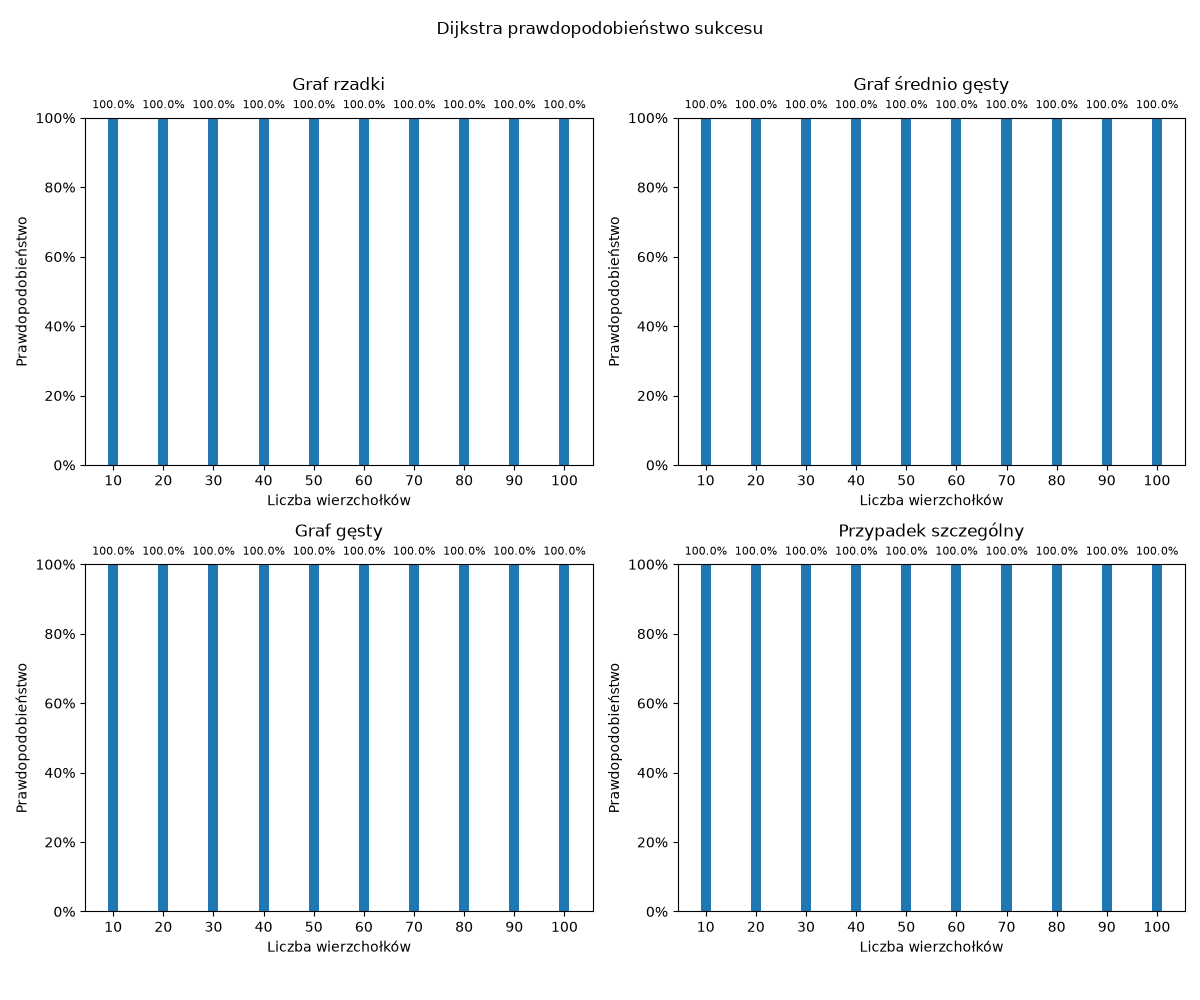
\includegraphics[width=0.95\columnwidth]{images/documentation/quantum_prob/quantum_prob_dijkstra_no_time_limit.png}
    \caption{Prawdopodobieństwo otrzymania poprawnego wyniku kwantowej wersji algorytmu Dijkstry bez limitu liczby operacji.}
    \label{fig:quantum_prob_dijkstra_no_time_limit}
\end{figure}

Na rys.~\ref{fig:quantum_prob_dijkstra_no_time_limit} przedstawiono skuteczność całego algorytmu Dijkstry bez ograniczenia liczby operacji wyszukiwania minimum.

Podobnie jak w przypadku samego algorytmu Dürra-Høyera, dla wszystkich rodzajów grafów otrzymano pełną poprawność.

\section{Zależność pomiędzy błędnym minimum a wynikiem algorytmu Dijkstry}

\begin{figure}[H]
    \centering
    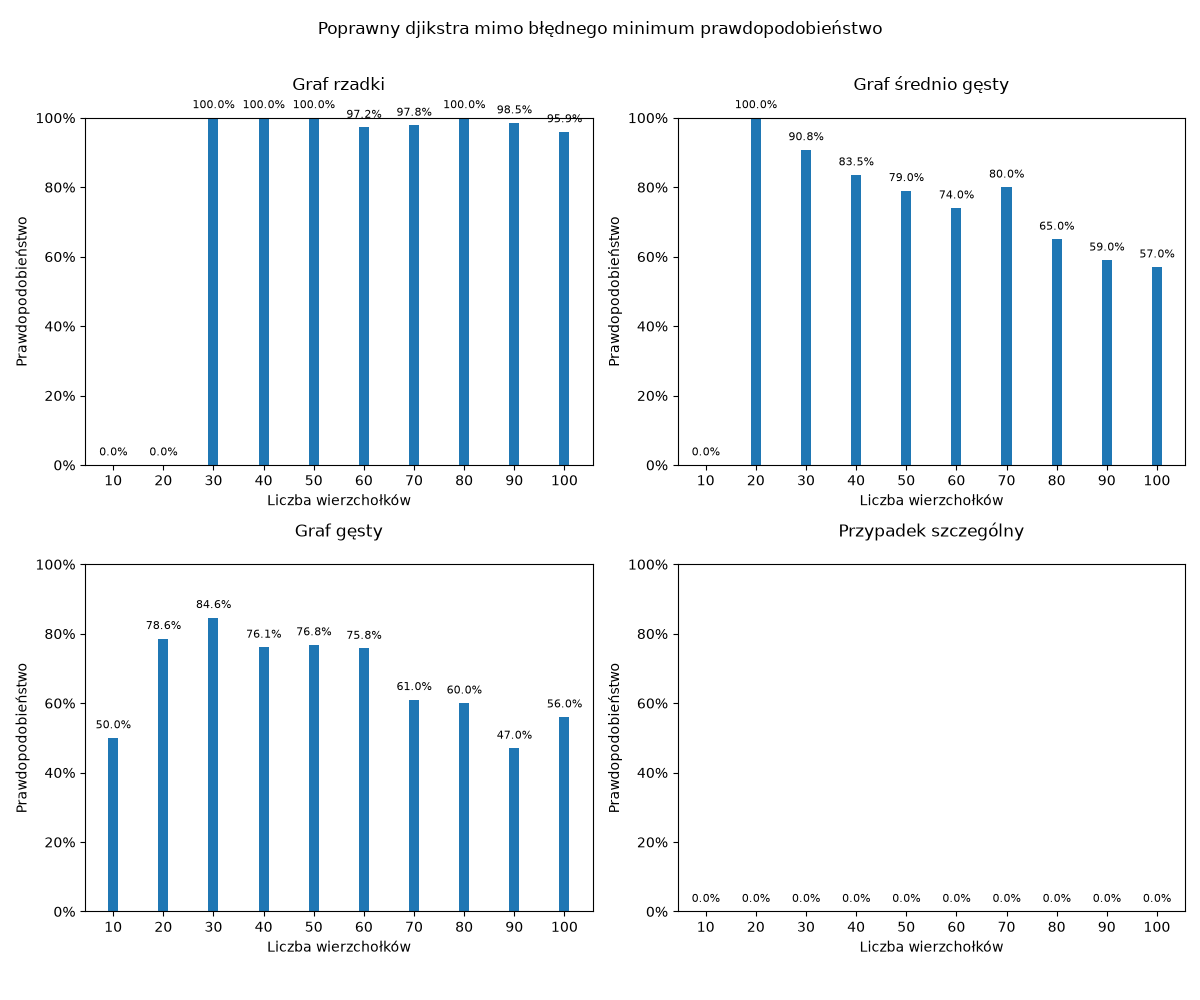
\includegraphics[width=0.95\columnwidth]{images/documentation/quantum_prob/quantum_prob_1vs_time_limit.png}
    \caption{Prawdopodobieństwo otrzymania poprawnego wyniku algorytmu Dijkstry pomimo wystąpienia błędnego minimum dla konfiguracji z limitem.}
    \label{fig:quantum_prob_1vs_time_limit}
\end{figure}

Na rys.~\ref{fig:quantum_prob_1vs_time_limit} przedstawiono przypadki, w których mimo wystąpienia błędnego minimum końcowy wynik algorytmu Dijkstry pozostaje poprawny.

\begin{figure}[H]
    \centering
    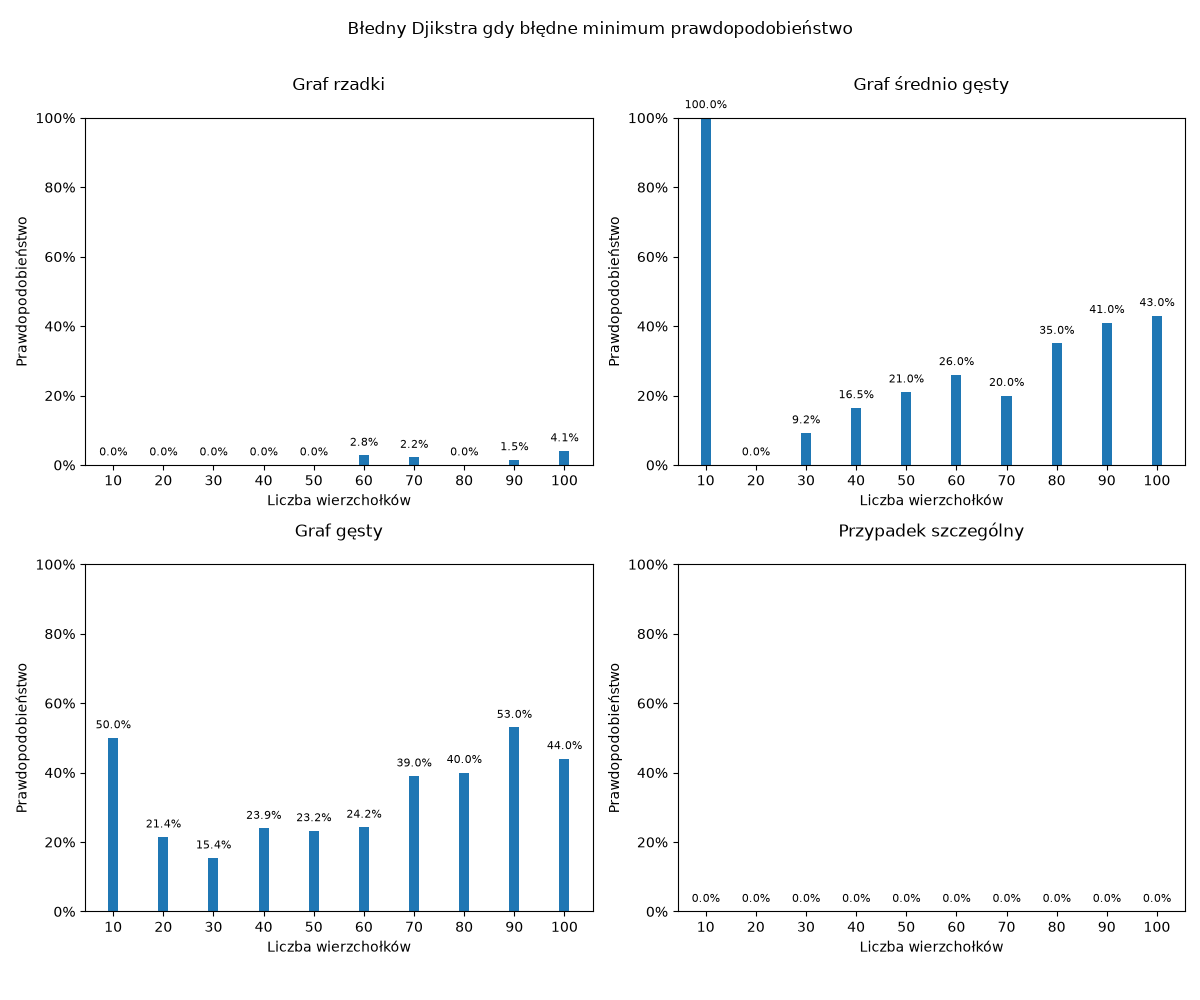
\includegraphics[width=0.95\columnwidth]{images/documentation/quantum_prob/quantum_prob_2vs_time_limit.png}
    \caption{Prawdopodobieństwo otrzymania błędnego wyniku algorytmu Dijkstry w przypadku wystąpienia błędnego minimum dla konfiguracji z limitem.}
    \label{fig:quantum_prob_2vs_time_limit}
\end{figure}

Rys.~\ref{fig:quantum_prob_2vs_time_limit} przedstawia tę samą zależność od strony błędnych wyników końcowych.

\subsection{Dlaczego błędne minimum nie zawsze prowadzi do błędnego wyniku}

W klasycznym algorytmie Dijkstry w każdej iteracji wybierany jest kolejny nieodwiedzony wierzchołek o najmniejszej odległości od aktualnego wierzchołka. Następnie wykonywana jest relaksacja jego krawędzi.

Aktualizacja odległości zachodzi tylko wtedy, gdy

\begin{equation}
d(v) > d(u) + w(u,v).
\end{equation}

W wersji kwantowej jeżeli algorytm wyszukiwania minimum Dürra-Høyera wybierze wierzchołek o nie najmniejszej odległości, nie oznacza to jeszcze, że końcowy wynik będzie niepoprawny. Dzięki relaksacji optymalne ścieżki między wierzchołkami mogą być poprawione. Oprócz tego w grafie może też istnieć wiele ścieżek prowadzących do tego samego wierzchołka. Relaksacje mogą wtedy doprowadzić do poprawnych wartości, nawet jeśli wcześniej wykonano niepoprawny wybór.
